\documentclass[11pt,letterpaper]{article}
\PassOptionsToPackage{hyphens}{url}
\usepackage[margin=.83in,top=.8in,bottom=.8in,headheight=15pt]{geometry}
\usepackage[T1]{fontenc}
\usepackage{lmodern,amsmath,amssymb,mathtools,bm,booktabs,array,graphicx,tikz}
\usetikzlibrary{arrows.meta,positioning,calc,decorations.pathreplacing,patterns}
\definecolor{ink}{HTML}{17344D}\definecolor{accent}{HTML}{087E8B}\definecolor{pale}{HTML}{EDF5F5}\definecolor{gold}{HTML}{AD6B19}
\providecommand{\dd}{\,\mathrm{d}}\providecommand{\R}{\mathbb{R}}
\providecommand{\E}{\mathbb{E}}\providecommand{\Var}{\operatorname{Var}}
\providecommand{\Cov}{\operatorname{Cov}}\providecommand{\diag}{\operatorname{diag}}
\providecommand{\norm}[1]{\left\lVert#1\right\rVert}
\providecommand{\abs}[1]{\left|#1\right|}
\usepackage{microtype,hyperref,fancyhdr,enumitem,amsthm,sectsty,needspace}
\allsectionsfont{\raggedright}
\hypersetup{colorlinks=true,linkcolor=ink,urlcolor=accent,pdfauthor={Zan Ahmad},pdftitle={Local image filters and learned classification / Lecture notes}}
\setlength{\parindent}{0pt}\setlength{\parskip}{6pt}\linespread{1.07}
\setlist{itemsep=3pt,topsep=4pt,leftmargin=*}
\emergencystretch=2em\clubpenalty=10000\widowpenalty=10000
\pagestyle{fancy}\fancyhf{}\fancyhead[L]{\small Mathematical Cardiology}\fancyhead[R]{\small Lecture 10}
\fancyfoot[L]{\footnotesize Zan Ahmad}\fancyfoot[R]{\footnotesize\thepage}\renewcommand{\headrulewidth}{.3pt}
\newtheorem{proposition}{Proposition}\newtheorem{theorem}{Theorem}\newtheorem{lemma}{Lemma}
\theoremstyle{definition}\newtheorem{definition}{Definition}\newtheorem{example}{Example}
\numberwithin{equation}{section}
\begin{document}
{\small\scshape Mathematical Cardiology\hfill Lecture 10}\par\medskip
{\raggedright\hyphenpenalty=10000\exhyphenpenalty=10000\LARGE\bfseries\color{ink} Local image filters and learned classification\par}\medskip
{\small Lecture notes}\par\bigskip
An image classifier can be decomposed into operations whose inputs and outputs have definite shapes. We shall follow an image through a local weighted sum, a nonlinearity, a spatial average and a fitted decision rule. This decomposition lets us distinguish the computations that resemble a convolutional network from the quantities that are actually learned. It also makes several checks possible before any accuracy is reported.

\section{An image, a mask, and a label}
\hypertarget{note-an-image-a-mask-and-a-label}{}\label{note:an-image-a-mask-and-a-label}
{\small \href{slides.html\#frame=specify-the-output\&step=1}{Slides for this section}}\par
Let $I\in\R^{16\times16}$ contain grayscale intensities. In this experiment each image contains a noisy synthetic ellipse. Its label is zero for an ellipse elongated horizontally and one for an ellipse elongated vertically, relative to the image axes. The target is a property assigned by the generator, not an anatomical or disease label.

Classification maps the whole image to one label. Segmentation maps image locations to labels, as in the threshold mask of the preceding lesson. Correctly classifying an image as wide therefore does not locate its boundary. Conversely, a mask can provide a useful shape measurement without being a classifier. The output type should be specified before an algorithm is selected.

The companion uses two fixed directional filters to turn the image into two numbers, then fits two class centers from training images. There is no fitted image normalization in this pipeline, unlike the standardized two-feature example in the previous calibration lesson. The two filter features already have matching numerical units. All image intensities are dimensionless synthetic values; physical pixel spacing and acquisition calibration are absent.
\section{A local weighted sum}
\hypertarget{note-a-local-weighted-sum}{}\label{note:a-local-weighted-sum}
{\small \href{slides.html\#frame=a-fixed-directional-kernel-figure\&step=1}{Slides for this section}}\par
The first kernel is
\begin{equation}K_x=\frac13\begin{pmatrix}-1&0&1\\-1&0&1\\-1&0&1\end{pmatrix},\qquad K_y=K_x^T.
\end{equation}
For a valid window beginning at $(i,j)$, its response is
\begin{equation}A^x_{ij}=\sum_{a=0}^2\sum_{b=0}^2(K_x)_{ab}I_{i+a,j+b}.\label{eq:filter-response}\end{equation}
Here $i,j$ run from $0$ to $13$. The kernel is not reversed, so the precise operation is a sliding dot product, often called convolution in neural-network software. Each response uses only the local $3\times3$ patch, and the same nine weights are used at every valid location. For an $N\times N$ image and $k\times k$ kernel with stride one and no padding, there are $N-k+1$ valid starts in either direction. Thus the $16\times16$ image produces a $14\times14$ map.

A patch with three rows $(0,0,1)$ gives response $3(1/3)=1$ under $K_x$. Reversing the rows to $(1,0,0)$ gives $-1$. A constant patch gives zero because the kernel weights sum to zero. Positive response therefore identifies an increase in intensity in one direction; it is neither a diagnosis nor a probability. With values in $[0,1]$, each column difference lies between $-1$ and $1$, so the response also lies in $[-1,1]$.
\begin{center}\begin{minipage}{.98\linewidth}\centering
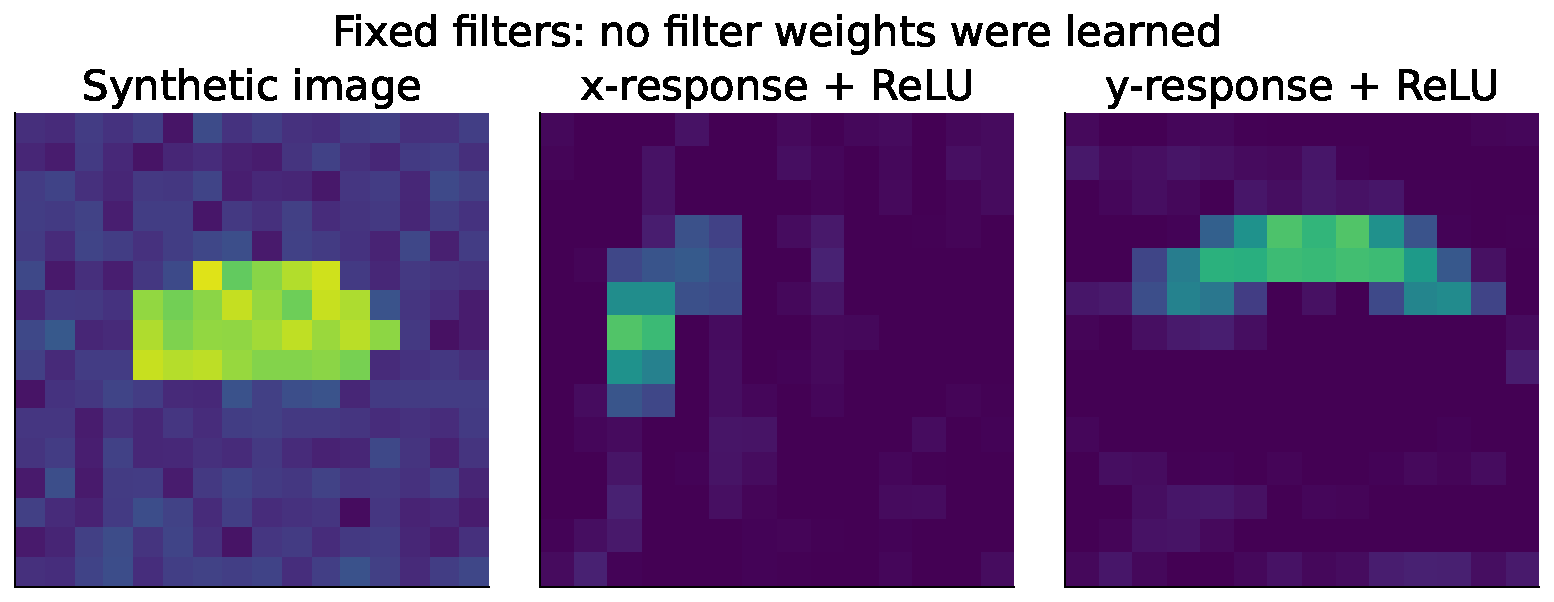
\includegraphics[width=.96\linewidth,height=.57\textheight,keepaspectratio]{image-filters.pdf}\par\smallskip
{\small Original sixteen-by-sixteen ellipse image and two fourteen-by-fourteen nonnegative directional response maps on a shared 0--1 color scale. Filters are fixed; none was learned.}
\end{minipage}\end{center}
\section{Nonlinearity, averaging, and information loss}
\hypertarget{note-nonlinearity-averaging-and-information-loss}{}\label{note:nonlinearity-averaging-and-information-loss}
{\small \href{slides.html\#frame=retain-only-positive-responses\&step=1}{Slides for this section}}\par
Apply the positive-part function, also called ReLU, to each response:
\begin{equation}B^x_{ij}=\max(A^x_{ij},0),\qquad B^y_{ij}=\max(A^y_{ij},0).
\end{equation}
Negative and positive responses no longer cancel. Global mean pooling then produces
\begin{equation}f_x(I)=\frac1{196}\sum_{i,j}B^x_{ij},\qquad
f_y(I)=\frac1{196}\sum_{i,j}B^y_{ij}.\end{equation}
The result is a point $f(I)=(f_x,f_y)$ in a two-dimensional feature space. Its coordinates are nonnegative and at most one for the supplied intensity range. Averaging discards the locations of the responses. Distinct images can therefore share the same feature pair, so a classifier using only these two numbers must give them the same prediction.

The operations yield useful exact checks. Constant images have zero features. Transposing a square image exchanges the two directional response maps up to transposition; since the average is unchanged by transposing a map,
\begin{equation}f(I^T)=(f_y(I),f_x(I)).\end{equation}
This matches the generator target: transposing a wide ellipse produces a tall one. A ninety-degree rotation also swaps wide and tall relative to the axes, so it is not a label-preserving augmentation. Pooling can reduce sensitivity to where a response occurs, but finite image boundaries, cropping and discarded negative responses prevent a claim of invariance to every translation or rotation.
\section{Fitted centers and learnable convolutional weights}
\hypertarget{note-fitted-centers-and-learnable-convolutional-weights}{}\label{note:fitted-centers-and-learnable-convolutional-weights}
{\small \href{slides.html\#frame=fit-the-output-rule\&step=1}{Slides for this section}}\par
The training sample contains eighty images generated with one seed; forty additional images generated with a different seed are held out. The class center is
\begin{equation}c_k=\frac1{n_k}\sum_{i:\,y_i=k}f(I_i),\qquad k\in\{0,1\},
\end{equation}
using training images only. A new image is assigned to the nearer center in ordinary squared Euclidean distance. Exact ties go to label zero in the implementation. The filters, ReLU and mean-pooling operations are fixed; only the centers are fitted. This is consequently a fixed-filter classifier, not a trained convolutional neural network.

A learned convolutional layer would adjust its kernel weights using training examples and a specified loss. Weight sharing matters even before considering how the weights are learned. One $3\times3$ filter has nine distinct weights, reused at $196$ valid image locations. A locally connected operation with separate weights at each of those locations would have $196\cdot9=1764$ weights for the same single output map, before adding biases. Our two kernels contain eighteen fixed coefficients; the fact that the coefficients are reused does not imply that they were trained.

A possible learned extension could use a scalar score $s_i=w^Tf_K(I_i)+b$ and minimize a loss such as the training mean of $(s_i-y_i)^2$, updating $K,w,b$. This merely specifies one possible optimization problem; it is not the companion algorithm, and the score need not be a calibrated probability. Demonstrating such an extension would require actual parameter updates, checks of the computation and independent evaluation.
\section{Evaluate the frozen rule}
\hypertarget{note-evaluate-the-frozen-rule}{}\label{note:evaluate-the-frozen-rule}
{\small \href{slides.html\#frame=the-held-out-image-counts-figure\&step=1}{Slides for this section}}\par
The default held-out confusion table, with true labels as rows, is
\[
\begin{array}{c|rr}
&\text{predicted wide}&\text{predicted tall}\\\hline
\text{true wide}&20&0\\
\text{true tall}&0&20
\end{array}
\]
All forty synthetic images are classified correctly. The result reflects a generator with a strong orientation difference that the chosen filters can represent. It is not evidence about medical-image variation or clinical targets. A constant wide prediction would correctly label twenty of these forty balanced cases.

The second comparison freezes the centers and changes the contrast parameter used to construct the same test masks. The tested contrast levels are $1$, $0.5$ and $0$, with observed accuracies $1$, $1$ and $0.5$. The noise realization and shape choices are reproducible under the fixed seed; the model is not refitted. At zero contrast the intended shape signal disappears, leaving background noise. The score at that level describes this finite realization; the absence of label information in the generator is the stronger reason no classifier can systematically recover orientation from that input distribution alone.
\begin{center}\begin{minipage}{.98\linewidth}\centering
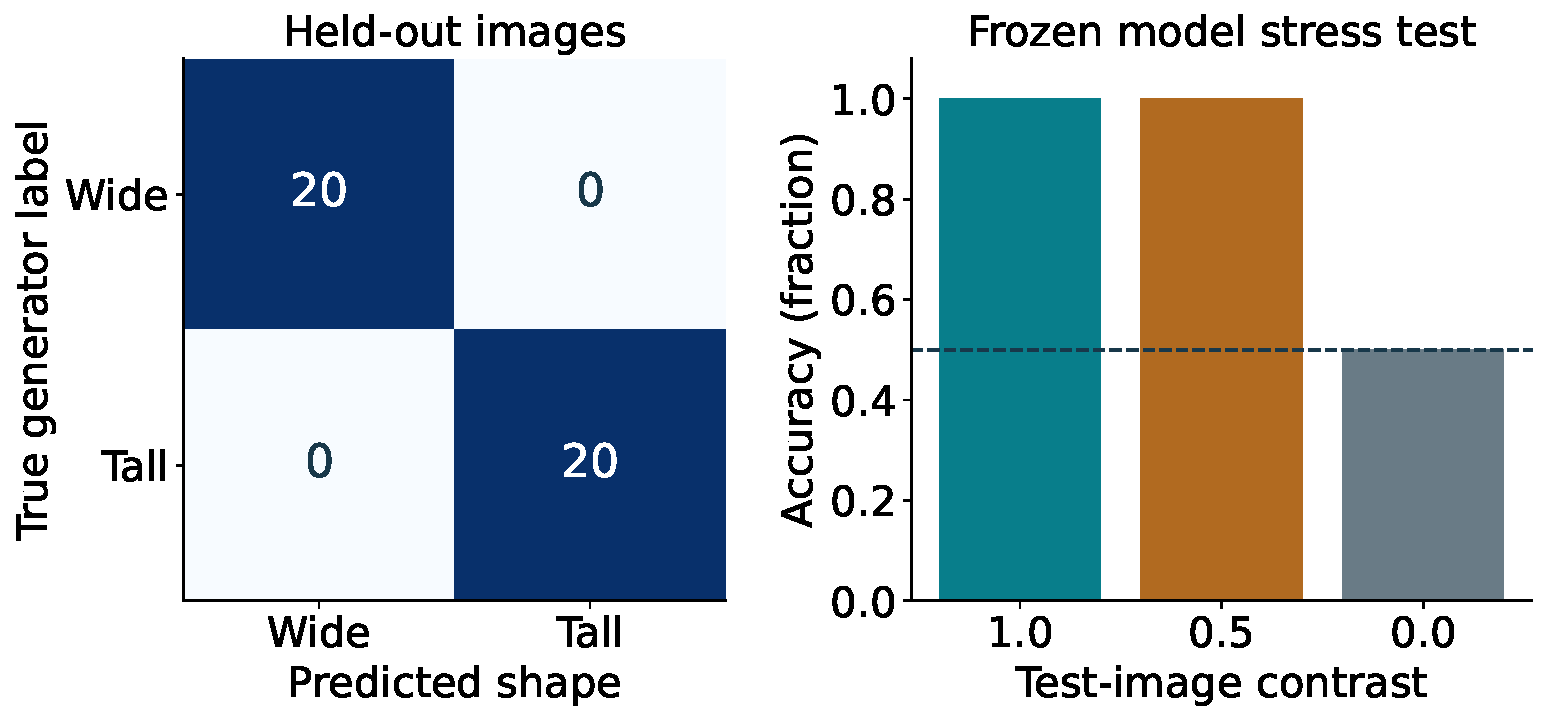
\includegraphics[width=.96\linewidth,height=.57\textheight,keepaspectratio]{image-evaluation.pdf}\par\smallskip
{\small Confusion counts on forty independent synthetic test images and a frozen-model contrast stress test. Labels describe image orientation. Perfect default performance is not clinical validation.}
\end{minipage}\end{center}
\section{Contrast, target transformations, and a defensible conclusion}
\hypertarget{note-contrast-target-transformations-and-a-defensible-conclusion}{}\label{note:contrast-target-transformations-and-a-defensible-conclusion}
{\small \href{slides.html\#frame=remove-the-signal-without-refitting\&step=1}{Slides for this section}}\par
A simple algebraic contrast calculation clarifies the stress test. If an image is replaced by $I'=aI+b\mathbf1$ with $a\geq0$, and there is no clipping or other alteration, zero-sum kernels give $A(I')=aA(I)$. Positive homogeneity of ReLU then gives $f(I')=af(I)$. Fixed class centers do not scale along with the test image, so this operation does not in general preserve nearest-center predictions. The actual generator changes the shape contrast while retaining noise and clipping values to $[0,1]$, so its stress images are not exactly this affine transformation. The algebra is a check on an idealized operation, not an assertion about every generated pixel.

For real data, the held-out unit must match the intended new case. Slices or repeated visits from one person may share information; a new-patient claim calls for separating people. A more complex network does not remove the need for appropriate labels, a frozen evaluation procedure and relevant failure tests. In a final model argument, give the target, the observations available at prediction time, the fitted quantities and the comparison that was actually performed. Here that conclusion is narrow and testable: two fixed directional features and training centers separate the specified ellipse orientations in the default synthetic test, and the result deteriorates when the orientation signal is removed.
\bigskip
\section*{Exercises}
\par\noindent\begin{minipage}{\linewidth}
\subsection*{MC10-E1. Slide a small filter}
A 4 by 4 image has four identical rows (0, 0, 0, 1). Use Kx from the notes, stride 1 and no padding.

\textbf{a} Find the output shape.

\end{minipage}\par\medskip
\textbf{b} Calculate all four responses.

\textbf{c} Apply ReLU and global mean pooling.

\par\noindent\begin{minipage}{\linewidth}
\subsection*{MC10-E2. What was learned?}
A pipeline uses two hand-set filters, ReLU, mean pooling and class centers estimated from training examples.

\textbf{a} Classify each component as fixed or fitted.

\end{minipage}\par\medskip
\textbf{b} Why is calling this a trained CNN misleading?

\textbf{c} What would a genuine convolutional-training extension need?

\par\noindent\begin{minipage}{\linewidth}
\subsection*{MC10-E3. Evaluate new cases}
On twenty balanced synthetic images, true-wide/pred-wide=\allowbreak{}9, true-wide/pred-tall=\allowbreak{}1, true-tall/pred-wide=\allowbreak{}3, true-tall/pred-tall=\allowbreak{}7.

\textbf{a} Calculate accuracy and the fraction of true-tall images recognized as tall.

\end{minipage}\par\medskip
\textbf{b} Compare with a classifier that always says wide.

\textbf{c} Explain why these results do not show reliable medical-image analysis.

\par\noindent\begin{minipage}{\linewidth}
\subsection*{MC10-E4. A valid project stress test}
A group labels images wide or tall, then rotates them 90 degrees as a supposed label-preserving augmentation.

\textbf{a} Identify and repair the label problem.

\end{minipage}\par\medskip
\textbf{b} Propose one predeclared stress test that does not intentionally change that target. State what stays frozen and which tested levels you will report.

\textbf{c} State three elements of the final project evidence chain.

\section*{References}
\noindent\begin{minipage}{\linewidth}
Zan Ahmad, Mathematical Cardiology syllabus, Fall 2023. Public PDF pages 1--2, Course Topics and Course Objectives.

\url{https://zanahmad.com/files/Fall_2023_HEART_Syllabus.pdf}
\end{minipage}\par\medskip
\noindent\begin{minipage}{\linewidth}
Zan Ahmad, original editable Mathematical Cardiology syllabus. Rendered export pages 2--3, Assignments \& Grading and Projects.

\end{minipage}\par\medskip
\noindent\begin{minipage}{\linewidth}
Stanford CS231n, Convolutional Neural Networks. Architecture Overview; Layers used to build ConvNets; Convolutional Layer; Pooling Layer; read 2026-11-14.

\url{https://cs231n.github.io/convolutional-networks/}
\end{minipage}\par\medskip
\noindent\begin{minipage}{\linewidth}
scikit-learn, Common pitfalls and recommended practices. Section 12.2, Data leakage; read 2026-11-14.

\url{https://scikit-learn.org/stable/common_pitfalls.html}
\end{minipage}\par\medskip
\end{document}
